%%\documentclass[12pt,letterpaper,doublespaced,ETD,dvips]{gt-ece-thesis}
\documentclass[12pt,letterpaper,doublespaced,ETD]{gt-ece-thesis} %taking dvips out enable pdf bookmark generation as well as the logo printing on the first page

\title{Target Tracking Using Residual Vector Quantization}
\author{Salman Aslam}
\copyrightyear{2011}
\graddate{20 June 2011}  
\approvaldate{June 2011}  

\addadvisor{Dr. Christopher F. Barnes}{Assoc. Professor, School of ECE}{Georgia Institute of Technology}
\addchair{Dr. David V. Anderson}{Assoc. Professor, School of ECE}{Georgia Institute of Technology}
\addreader{Dr. Aaron F. Bobick, Co-advisor}{Professor, School of Interactive Computing}{Georgia Institute of Technology}
\addreader{Dr. Vijay Madisetti}{Professor, School of ECE}{Georgia Institute of Technology}
\addreader{Dr. Patricio Vela}{Asst. Professor, School of ECE}{Georgia Institute of Technology}
\addreader{Dr. Santanu Dey}{Asst. Professor, School of ISYE}{Georgia Institute of Technology}


\bibfiles{f:/salman/work/writing/MyCitations}

\titlepagetrue
\figurespagetrue
\tablespagetrue
\contentspagetrue
\symbolspagefalse
\glossarypagefalse 
\bibpagetrue
\mastersthesisfalse 
\multivolumefalse
\singlespacednotestrue


\usepackage{graphicx, subfigure, verbatim}
\usepackage{insfig}
\usepackage{url}
\usepackage{multirow}
\usepackage{hyperref}
\usepackage{longtable}
\usepackage[usenames,dvipsnames]{color}
\definecolor{light-gray}{gray}{0.95}
\usepackage{amsmath,epsfig,verbatim,listings}
\lstset{breaklines=true,breakindent=0pt,
        prebreak=\mbox{\tiny$\searrow$},
        postbreak=\mbox{{\color{blue}\tiny$\rightarrow$}},
	tabsize=2,
linewidth=1.1\linewidth,
xleftmargin=-0.8in,
basicstyle=\tiny,
numbers=left,
frame=single,
captionpos=t,
title=\lstname,
backgroundcolor=\color{light-gray}}


\setchaptertocdepth{2}
\setappendixtocdepth{2}

\settocstring{Table of Contents}
\setlofstring{List of Figures}
%\setlotstring{List of Tables}
\setbibstring{References}
\setindstring{Index}
\setdedstring{Dedication}
\setglostring{List of Terms}
\setchpstring{Chapter}
\setappstring{Appendix}
\setprtstring{Volume}
\setabsstring{Summary}
\setlosstring{List of Symbols}
\setackstring{Acknowledgment}

\setfrontpagestyle{plain}
\setbodypagestyle{plain}
\setendpagestyle{plain}

\pagestyle{plain}
\bibliographystyle{ieeetr}
%\definecolor{darkgreen}{rgb}{0,0.5,0}
\newcommand{\Ntrg}{\big[N_{t=1, m=1} + \lambda \big] + \big[N_{t=1, m=2} + \lambda \big] + \ldots + \big[N_{t=1, m=M} + \lambda \big]}
\newcommand{\jointcnt}{\sum\limits_{n_{trg}=1}^{N_{trg}}I(X_t=x_t, X_{t-1}=x_{t-1})}
\newcommand{\singlecnt}{\sum\limits_{n_{trg}=1}^{N_{trg}}I(X_{t-1}=x_{t-1})}
\newcommand{\singlep}{p(X_{t-1}=x_{t-1})}
\newcommand{\singlepone}{p(X_{t-1}=1)}
\newcommand{\singleptwo}{p(X_{t-1}=2)}
\newcommand{\singlepM}{p(X_{t-1}=M)}
\newcommand{\condp}{p(X_t=x_t | X_{t-1}=x_{t-1})}
\newcommand{\jointp}{p(X_t=x_t, X_{t-1}=x_{t-1})}
\newcommand{\KmeansOuterSum}{\sum\limits_{k=1}^K}
\newcommand{\KmeansInnerSum}{\sum\limits_{{i=1 \atop x_i \in \mathcal{K}_k}}^N}
\newcommand{\KmeansSum}{\KmeansOuterSum \KmeansInnerSum}
\newcommand{\RVQInnerSum}{\sum\limits_{{i=1 \atop g_i \mapsto m_{\tau, s}}}^N}
\newcommand{\RVQOuterSum}{\sum_{s=1}^S}
\newcommand{\RVQsum}{\KmeansOuterSum \sum\limits_{{i=1 \atop g_i \in \mathcal{K}_k}}^N}
\newcommand{\KmeansInner}{{(x_i - \mu_k)}^2}
\newcommand{\RVQinner}{            {(x_i  - \hat{\mu}^{(k)})}^2}
\newcommand{\RVQinneralternate}{{(g_i - m_\tau^{(k)})}^2}
\newcommand{\RVQinneralternatealternate}{{(g_i - m_{\tau, s})}^2}
\newcommand{\KmeansError}{\KmeansSum \KmeansInner}
\newcommand{\RVQerror}     {\KmeansSum \RVQinner}
\newcommand{\RVQerroralternate}{\RVQsum \RVQinneralternate}
\newcommand{\RVQunit}{x_i -\bigg(\sum_{t=1}^Tm^{(k)}_t\bigg)}
\newcommand{\RVQequivalentCodevector}{\sum_{t=1 }^Tm^{(k)}_t}
\newcommand{\RVQequivalentCodevectorBroken}{\sum_{t=1 \atop t \neq \tau}^Tm^{(k)}_t+ m^{(k)}_\tau}
\newcommand{\RVQmultipleKmeans}{x_i -\bigg(\RVQequivalentCodevectorBroken\bigg)}
\newcommand{\RVQmultipleKmeansone}{x_i -\sum_{t=2}^Tm^{(k)}_t+ m^{(k)}_1\bigg)}
\newcommand{\RVQmultipleKmeansonealternate}{\bigg(x_i -\sum_{t=1 \atop t \neq \tau}^Tm^{(k)}_t\bigg) - m^{(k)}_\tau}
\newcommand{\RVQmultipleKmeanstwo}{x_i -\bigg(\sum_{t=1 \atop t \neq 2}^Tm^{(k)}_t+ m^{(k)}_2\bigg)}
\newcommand{\RVQmultipleKmeansT}{x_i -\bigg(\sum_{t=1}^{T-1}m^{(k)}_t+ m^{(k)}_2\bigg)}
\newcommand{\EucMatrix}
{
\left[
\begin{array}{lll}
r_{11} & r_{12} & t_x \\ 
r_{21} & r_{22} & t_y \\ 
0 & 0 & 1 \\ 
\end{array}
\right]
}	

\newcommand{\SimMatrix}
{
\left[
\begin{array}{lll}
sr_{11} & sr_{12} & t_x \\ 
sr_{21} & sr_{22} & t_y \\
0 & 0 & 1 \\ 
\end{array}
\right]
}

\newcommand{\AffMatrix}
{
\left[
\begin{array}{lll}
a &b & t_x \\ 
c & d & t_y \\
0 & 0 & 1 \\
\end{array}
\right]
}

\newcommand{\ProjMatrix}
{
\left[
\begin{array}{lll}
h_{11} & h_{12} & h_{13} \\ 
h_{21} & h_{22} & h_{23} \\ 
h_{31} & h_{32} & h_{33} \\ 
\end{array}
\right]
}

\newcommand{\RotMatrixTheta}
{
\left[
\begin{array}{rr}
\cos(\theta) & -\sin(\theta) \\ 
\sin(\theta) & \cos(\theta) \\ 
\end{array}
\right]
}

\newcommand{\RotMatrixPhi}
{
\left[
\begin{array}{rr}
\cos(\phi) & -\sin(\phi) \\ 
\sin(\phi) & \cos(\phi) \\ 
\end{array}
\right]
}

\newcommand{\RotMatrixminusPhi}
{
\left[
\begin{array}{rr}
\cos(-\phi) & -\sin(-\phi) \\ 
\sin(-\phi) & \cos(-\phi) \\ 
\end{array}
\right]
}


\newcommand{\EigenvalueMatrix}
{
\left[
\begin{array}{cc}
\lambda_1 & 0\\
0 & \lambda_2
\end{array}
\right]
}

\newcommand{\bigMatrix}
{
s \left[
\begin{array}{cc}
 (r)(a) + b &  (r)(d) - c \\
 (r)(c) - d &  (r)(b) + a
\end{array}
\right]
}


\newcommand{\bigMatrixTwo}
{
\left[
\begin{array}{cc}
(\lambda_2) p + (\lambda_1) q & (\lambda_2) s  - (\lambda_1) r \\
(\lambda_2) r  - (\lambda_1) s & (\lambda_2) q + (\lambda_1) p
\end{array}
\right]
}
\newcommand{\dr}{(\mathbf{x}_i-\boldsymbol\mu_k)^T(\mathbf{x}_i-\boldsymbol\mu_k) + \lambda({Q_{\textrm{max}}-Q_i})}

%\begin{document}
%\begin{FrontMatter}
%\contents %generates the TOC, LOF, and LOT
%\end{FrontMatter}
%\begin{Body}

%@@@@@@@@@@@@@@@@@@@@@@@@@@@@@@@@@@@@@@@@@@@@@@@@@@
\chapter{Tracking Methods}
\label{chap_TRK}	
%@@@@@@@@@@@@@@@@@@@@@@@@@@@@@@@@@@@@@@@@@@@@@@@@@@
Visual tracking is an important and difficult area of computer vision that has received a lot of attention in the literature.  Refer to~\cite{2006_JNL_SURVEYtrk_Trucco, 2006_JNL_SURVEYtrk_Yilmaz, 2008_REP_SURVEYtrk_Cannons} for surveys on this topic.

The biggest challenge in tracking is difficulty in handling changes in target appearance~\cite{2008_JNL_subspaceTRK_Ross}.  Intrinsic variations include pose variation and shape deformations.  Extrinsic variations include illumination change, camera motion, camera viewpoint and occlusions.  In order to simplify the process of tracking, it is common to make certain assumptions.  These assumptions fall under two broad categories:


								\begin{figure}[t]
								\center
								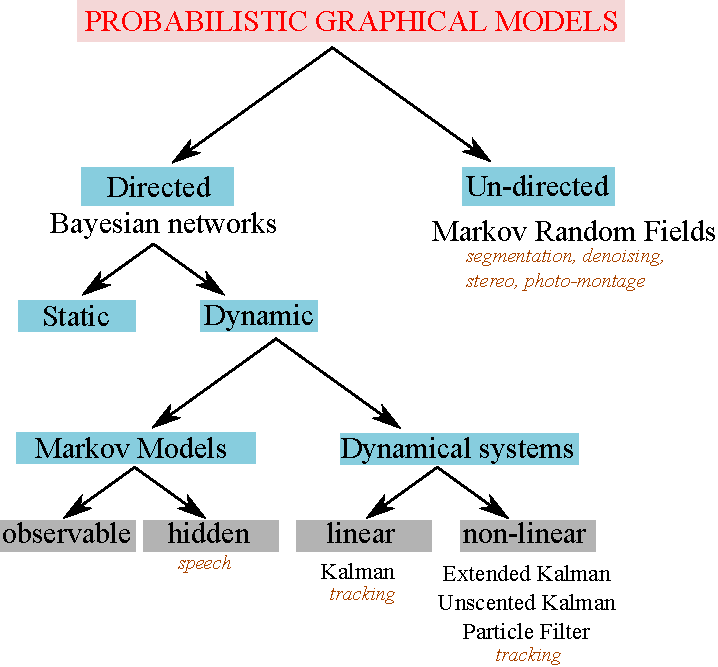
\includegraphics[width=0.7\textwidth]{thesis/PRML_PGM_overview.pdf}
								\caption{Tracking, big picture.}
								\label{fig:TRK_big_picture}
								\end{figure}


\begin{itemize}
\item \underline{Assumptions related to camera}.  A common assumption, in particular in surveillance applications, is a stationary camera that allows for background maintenance.  Known camera-motion is also used although it is less common.
\item \underline{Assumptions related to target}.  These assumptions include constant velocity, constant acceleration, coherent motion (all parts of the target move together) and motion along a straight path.
\end{itemize}

								\begin{figure}[t]
								\center
								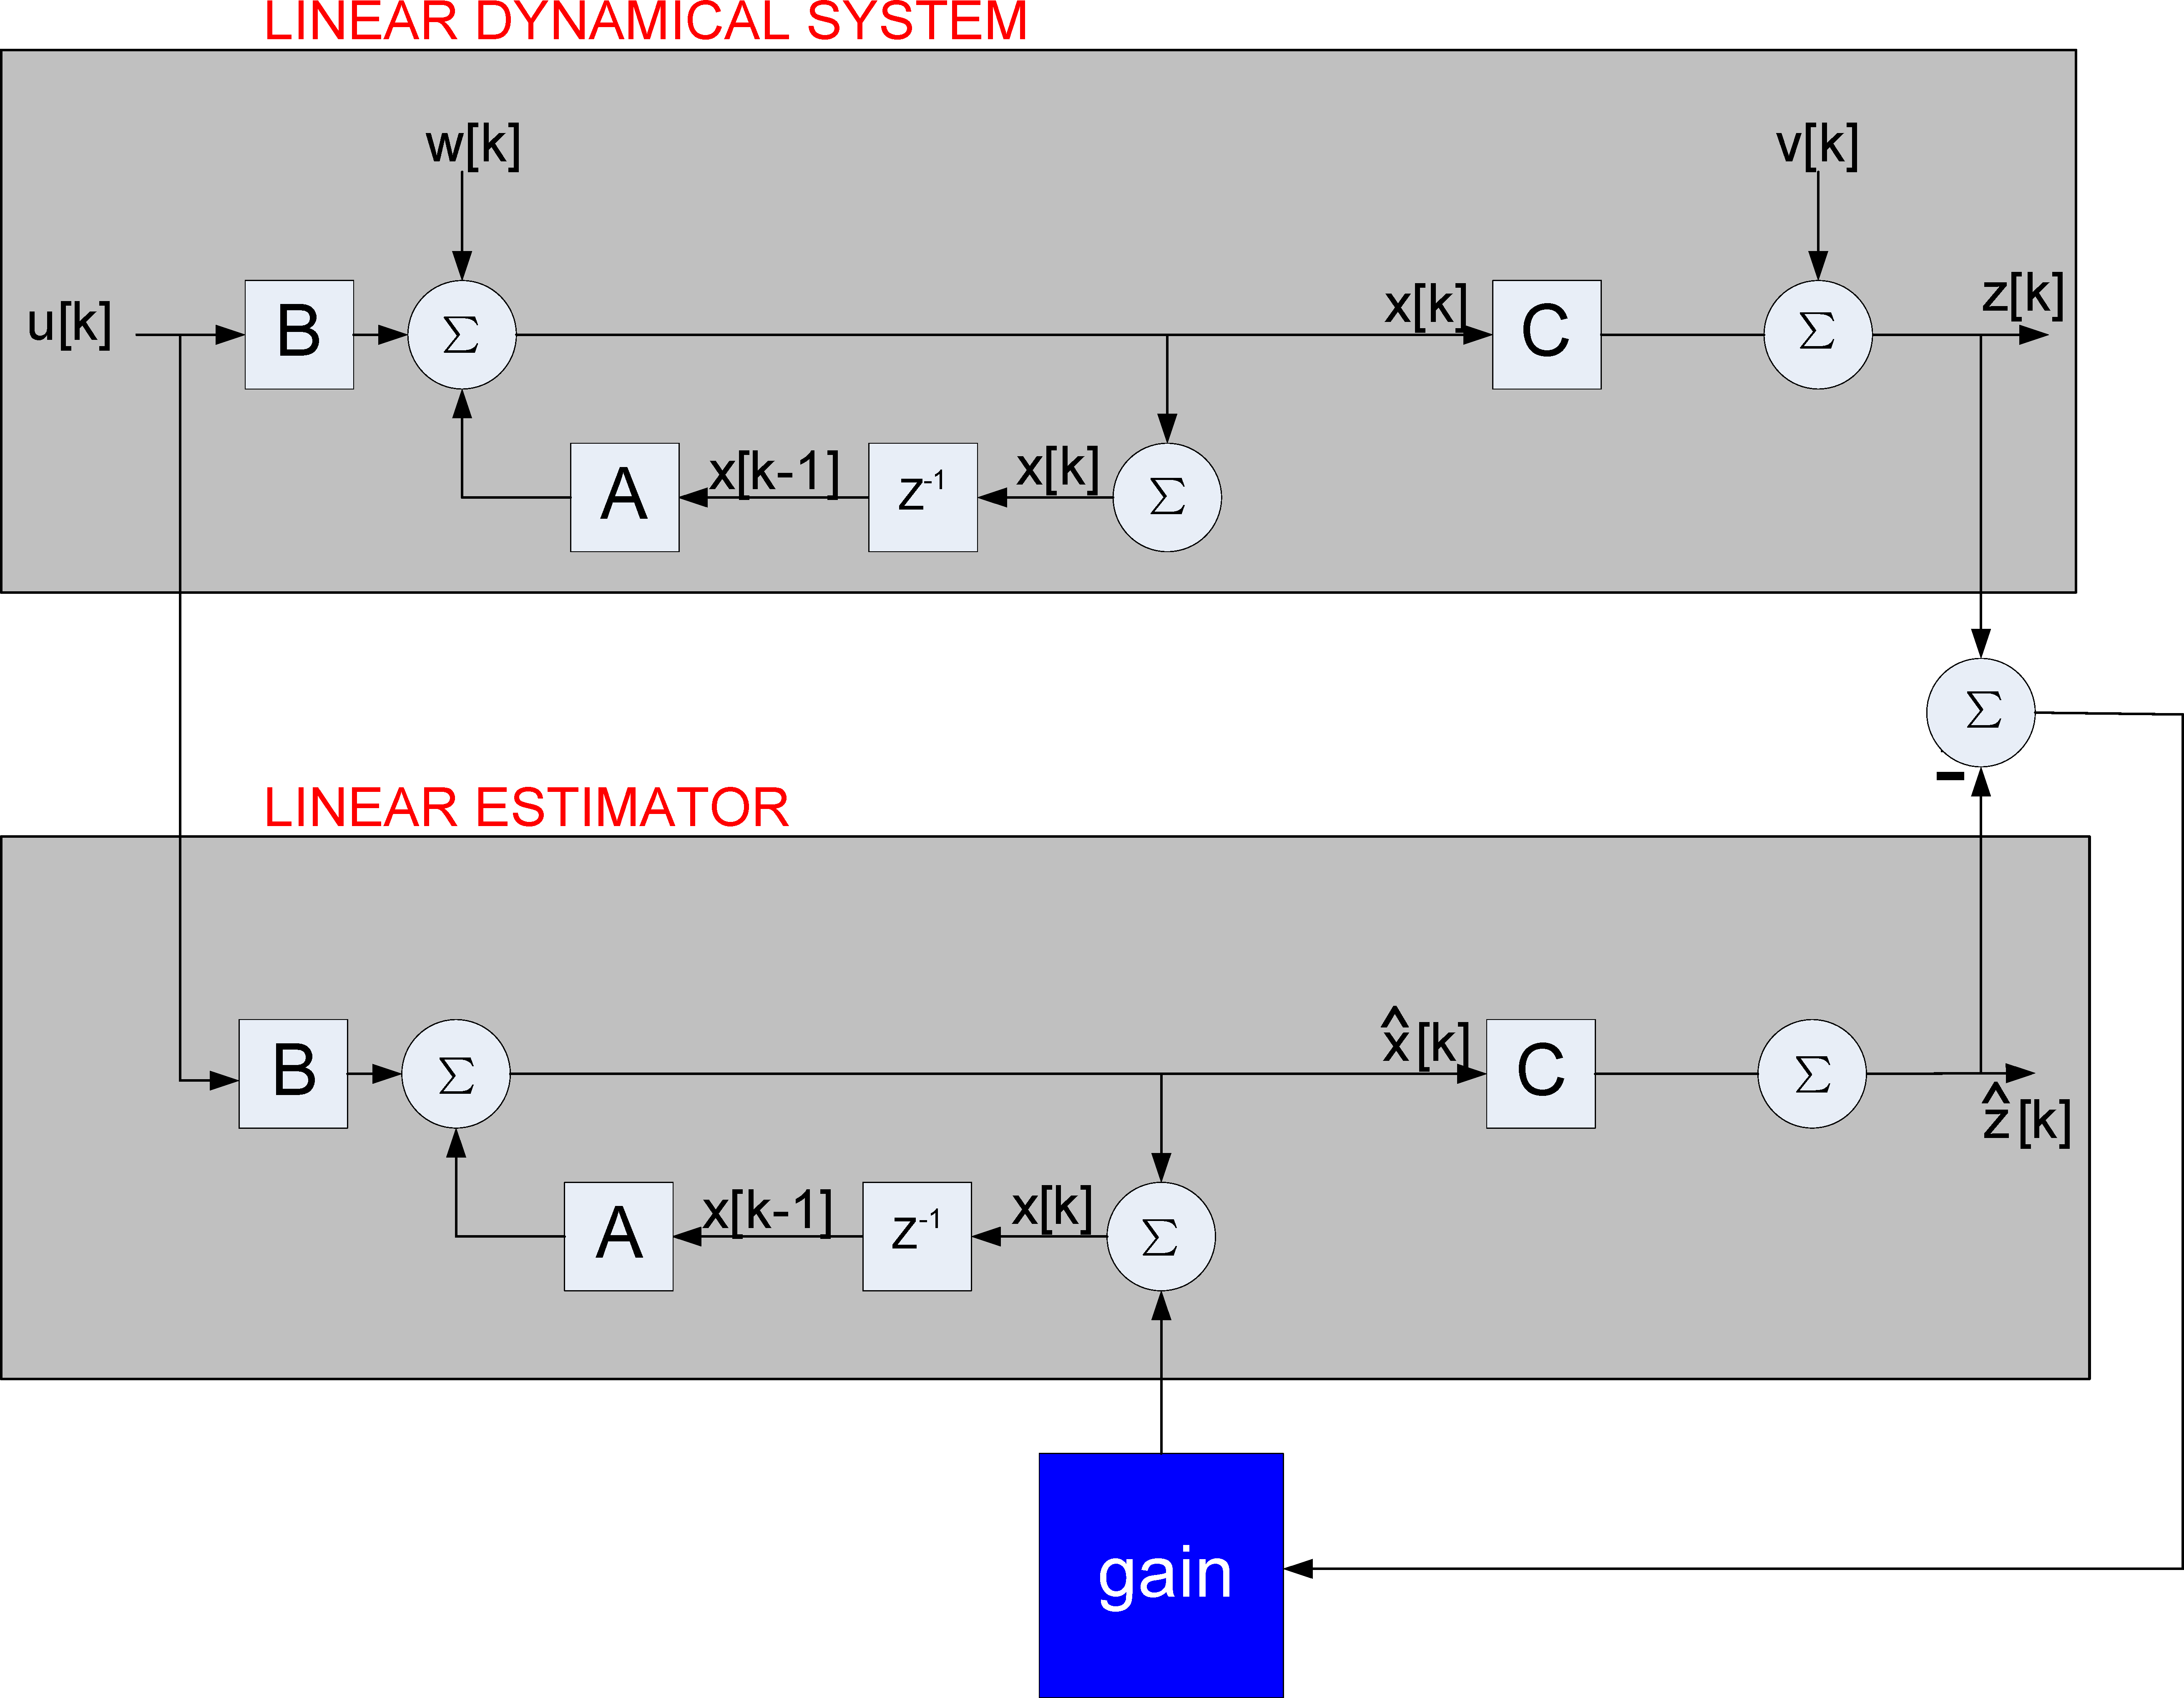
\includegraphics[width=1.0\textwidth]{thesis/TRK_LinearEstimator_blockDiagram.pdf}
								\caption{Linear estimator.  The gain block is called the \emph{Kalman gain} for the Kalman filter.}
								\label{TRK_overviewDiagram}
								\end{figure}

Furthermore, several pre-processing steps may be required before tracking can be initiated.  These include stabilization for video registration, normalization, downsampling, background modeling and feature extraction.  Refer to~\cite{1999_CNF_Wallflower_Toyama} for a survey on background modeling. Commonly used features include corners, area, color, intensity distributions, contour descriptors and depth.

								\begin{figure}[t]
								\center
								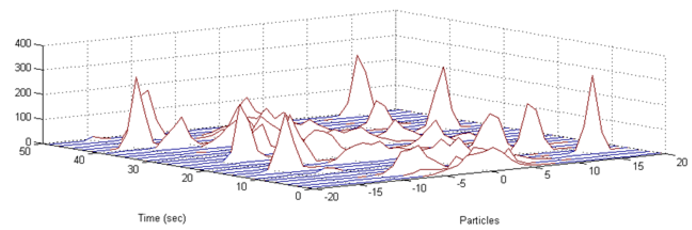
\includegraphics[width=1.0\textwidth]{thesis/TRK_ParticleFilter_multimodalPDF_part.png}
								\caption{Tracking using a particle filter.  Notice that the density is non-Gaussian and multi-modal.}
								\label{fig:particle_filter_multi_modal_density}
								\end{figure}



%#######################		
\section{Bayesian estimation}
%#######################
A commonly used formulation for tracking is based on Bayesian estimation.  In this framework, target kinematics are modeled as the latent states of a time-dynamic system~\cite{2002_JNL_PF_Arulampalam}.  Time-dynamic systems are based on two models: (a) \emph{state prediction model}, ${f_t:R^D \times R^D \rightarrow R^D}$, describing state evolution, and (b) \emph{observation model}, ${h_t:R^N \times R^N \rightarrow R^N}$, relating observations to the states.  These models are described as,

\begin{align}
\mathbf{x}_t &= f_t(\mathbf{x}_{t-1}, \mathbf{v}_{t-1}) \notag\\
\mathbf{z}_t &= h_t(\mathbf{x}_t, \mathbf{n}_t)
\label{Eq:TDS}
\end{align}

$\mathbf{v} \in R^D$ is an independent, identically-distributed (IID) process noise sequence.  $\mathbf{n} \in R^N$ is an IID measurement noise sequence.  The goal is to find the estimate of the state $\mathbf{x}_t$ at time $t$, based on all observations $\mathbf{Z}_t={\{\mathbf{z}_i, i=1,...,T\}}$.   $\mathbf{z}_t$ is the observation vector at time $t$.  

At this point, it is interesting to place the process of tracking in the bigger picture of probabilistic graphical models, as shown in Figure~\ref{fig:TRK_big_picture}.  Mathematically, hidden Markov models (HMMs) can also be written using evolution and observation models even though the method was developed independently of time dynamic systems \cite{2007_BOOK_PRML_Bishop}.  

This two stage model lends itself well to Bayesian inference \cite{2002_JNL_PF_Arulampalam}.  The reason is that observations can be used as evidence to modulate the prior distribution on the states.  We can then infer the posterior distribution on the states using Bayes' Rule.  Mathematically, the Chapman Kolmogorov equation predicts the next state by combining information from the state prediction model $p(\mathbf{x}_t| \mathbf{x}_{t-1})$ and all previous observations $\mathbf{Z}_{t-1}$.  %This is given in Equation~\ref{Eqn:TRK_prediction}.

{%\Large
\begin{equation}
\begin{array}{lllllllll}
{\color{darkgreen}p(x_t|Z_{t-1})} &= \frac{p(x_t, Z_{t-1})}{p(Z_{t-1})}\\
&=\frac{\int p(x_t, x_{t-1}, Z_{t-1})dx_{t-1}}{p(Z_{t-1})}\\
&=\frac{\int {\color{Cyan}p(x_t|x_{t-1}, Z_{t-1})}p(x_{t-1},Z_{t-1})dx_{t-1}}{p(Z_{t-1})}\\
&=\frac{\int {\color{Cyan}p(x_t|x_{t-1})}{\color{red}p(x_{t-1}|Z_{t-1})}p(Z_{t-1})dx_{t-1}}{p(Z_{t-1})}\\
&=\int {\color{Cyan}p(x_t|x_{t-1})}{\color{red}p(x_{t-1}|Z_{t-1})}dx_{t-1}
\end{array}
\label{Eqn:TRK_prediction}
\end{equation}
}


%\begin{equation}
%p(x_k|\textbf{Z}_{k-1})=
%\int{p(\mathbf{x}_k| \mathbf{x}_{k-1})p(\mathbf{x}_{k-1}|\mathbf{Z}_{k-1})}d\mathbf{x}_{k-1}
%\label{eq:ChapmanKolmogorov}
%\end{equation}  

In the second step, the observation $\mathbf{z}_t$ at time $t$ and the predicted state $\mathbf{x}_t$ can be used to compute the posterior estimate of the state $\mathbf{x}_t$ using %Equation~\ref{Eqn:TRK_update}.


{%\large
\begin{equation}
\begin{array}{lllllllll}
{\color{red}p(x_t | Z_t)} &= \frac{p(x_t, Z_t)}{p(Z_t)}\\
&= \frac{p(x_t, z_t, Z_{t-1})}{p(z_t, Z_{t-1})}\\
&= \frac{{\color{blue}p(z_t|x_t,Z_{t-1})}p(x_t, Z_{t-1})}{p(z_t|Z_{t-1})p(Z_{t-1})}\\
&= \frac{{\color{blue}p(z_t|x_t)}{\color{darkgreen}p(x_t|Z_{t-1})}p(Z_{t-1})}{p(z_t|Z_{t-1})p(Z_{t-1})}\\
&= \frac{{\color{blue}p(z_t|x_t)}{\color{darkgreen}p(x_t|Z_{t-1})}}{\int{p(z_t|x_t){\color{darkgreen}p(x_t |Z_{t-1})}}dx_t}
\end{array}
\label{Eqn:TRK_update}
\end{equation}
}



%\begin{equation}
%p(\mathbf{x}_k|\textbf{Z}_k)	= \frac{p(\mathbf{z}_k|\mathbf{x}_k)p(\mathbf{x}_k |\textbf{Z}_{k-1})   }{p(\mathbf{z}_k| \textbf{Z}_{k-1})}
%\label{eq:posterior}			
%\end{equation}

Equations~\ref{Eqn:TRK_prediction} and~\ref{Eqn:TRK_update} form the optimal Bayesian solution for the recursive propagation of the posterior density.  This problem can be solved analytically using the closed-form Wiener-Kalman linear Minimum Mean Square Estimate (MMSE) in Gaussian noise \cite{1964_JNL_BayesianEstimation_Ho, 1993_BOOK_SSP_Kay}.  Non-analytical methods, such as grid-based methods, can be used if the state space is discrete and consists of a finite number of states.  For non-linear models, the Extended Kalman Filter (EKF) computes the Jacobian for a Taylor Series expansion of the system and observation models about the current state \cite{2005_Misc_KalmanFilterComparison_Orderud}.  Recently, the Unscented Kalman Filter (UKF) has been replacing the EKF in a wide range of applications.  The UKF, instead of explicitly computing the Jacobian, computes a set of points that capture the true mean and covariance of the prior.  When propagated through the non-linear system, these points capture the posterior mean and covariance \cite{1997_CNF_UKF_Julier}.  As a result, the UKF estimates the posterior mean and covariance accurately to at least the second-order Taylor Series expansion.  The EKF on the other hand achieves only first-order accuracy \cite{2004_CNF_SigmaPointKalman_Merwe, 2000_CNF_UKF_Wan}.  More recently, particle filters which use point mass representations for probability densities and are based on stochastic sampling have been introduced in the visual tracking literature \cite{1993_JNL_ParticleFilter_Gordon, 2001_JNL_PFjumpMarkov_Doucet}.  A primary difference between the UKF and the particle filter is that the former is based on deterministic sampling while the latter is based on stochastic sampling.  Particle filters offer an additional advantage of being able to handle arbitrary densities as shown in Figure~\ref{fig:particle_filter_multi_modal_density}.  However, since the particle filter uses non-parametric densities with no functional representations, its computations do not scale well as the dimensionality increases~\cite{2004_CNF_TrackingPeople_Zhao}.  

A variety of particle filters have now been introduced.   According to~\cite{2002_JNL_PF_Arulampalam}, sequential Monte Carlo (SMC) filtering has been called particle filtering~\cite{1999_CNF_PF_carpenter}, bootstrap filtering~\cite{1993_JNL_ParticleFilter_Gordon}, the condensation algorithm~\cite{1998_JNL_Condensation_IsardBlake}, interacting particle approximations~\cite{1999_JNL_PF_Crisan, 1999_BK_PF_Moral} and survival of the fittest~\cite{1995_CNF_PF_Kanazawa}.

  
%The particle filter formulation is generally similar to the method which is used for the Kalman Filter.  A prediction step is followed by an update step, which is followed by a prediction step, and so on.  The update equation at time $t$ for a state $x_t$ given all observations $z_T$ involves computing the posterior density $p(x_t | Z_t)$.  In this case, the posterior density factors into a likelihood at time $t$, $p(z_t|x_t)$ and a prior density, $p(x_t|Z_{t-1})$, 
%
%
%
%
%The prior density can be computed using the Chapman-Kolmogorov equation by introducing the nuisance parameter $x_{t-1}$,
%
%
%$p(x_t|x_{t-1})$ is computed using the motion model while $p(x_{t-1}|Z_{t-1})$ is the posterior density from the previous time step, $t-1$.
%
%
%Visual tracking in clutter is difficult using the Kalman filter since clutter can typically give rise to several competing observations which encourage a non-unimodal density and gaussian densities cannot represent simultaneous alternative hypotheses~\cite{1998_JNL_Condensation_IsardBlake}.  Moreover 


%However, currently, the most popular version is the SIR (Sampling Importance Resampling) filter \cite{2009_BOOK_PF_Doucet}.  The resampling step prevents the posterior from collapsing to a single point.  The steps involved in computing the solution to this filter are summarized below:

%\begin{itemize}
%\item \textbf{Sampling with replacement.}  This step is carried out to guarantee that the algorithm runs within given computational resources.  $N$ samples are chosen from the set $\mathbf{s}_{k-1}^n$, each element being chosen with probability $\pi_{k-1}^n$.  %a sampling with replacement st from $p(\mathbf{x}_k | \mathbf{x}_{k-1})$
%\item Calculate particle weights from the likelihood, $\mathbf{w}_k = p(\mathbf{z}_k|\mathbf{x}_k)$
%\item Calculate the posterior ($p(\mathbf{x}_k | \mathbf{x}_{k-1})$.  First normalize weights.  Then resample using normalized-weights and sampled-prior. 
%\end{itemize}









%#######################		
\section{Traditional methods}
%#######################


\subsection{Point tracking}
%==========================
The problem of point tracking in the field of Computer Vision is similar to the problem of point tracking in the field of Radar Signal Processing.  This problem has been extensively studied and is also known as the \emph{data association} problem.  In Computer Vision, an additional pre-processing step, \emph{interest-point detection}, is required to extract points of interest from the scene.  Point tracking methods can be broadly categorized into statistical methods and deterministic methods.

There are three main statistical methods for point tracking.  The \emph{Probability Data Association Filter (PDAF)} provides a computationally efficient method of data association for single targets \cite{1975_JNL_PDAF_BarShalom}.  It is largely based on the Kalman Filter.  However, it has a mechanism of accounting for clutter.  The primary difference between the Kalman filter and the PDAF algorithm is in the computation of the innovations process during the update stage.  For multiple targets, this algorithm is generalized by the \emph{Joint Probability Data Association Filter (JPDAF)}~\cite{1983_JNL_JPDAF_Fortmann}.  The \emph{Multiple Hypothesis Tracker (MHT)} handles multiple targets in non-linear conditions~\cite{1979_JNL_MTT_Reid}.  MHT requires ever-expanding memory as more and more data is processed.  However, computationally practical versions of MHT have been reported \cite{1996_JNL_EfficientMHT_Cox, 1994_CNF_MLPMHT_Streit}.  It may be noted that a carefully designed MHT can provide better performance than the PDAF and JPDAF algorithms \cite{2009_JNL_PDAF_Barshalom}.  Additional details can be found in a survey by Cox \cite{1993_JNL_SURVEYcorresp_Cox}.  

Statistical methods have a number of shortcomings.  First, the assumption that points move independently is not always valid.  Second, measurements are not always distributed normally around their predicted position.  Third, there are a number of parameters to estimate, such as apriori probabilities for false measurements and missed detections.  And finally, statistical methods can be computationally demanding \cite{2001_JNL_MotionCorrespondence_Veenman}.  To deal with these shortcomings, a number of researchers have worked on deterministic methods for point tracking.

Most deterministic methods minimize a cost of associating a target to an observation.  This correspondence cost is usually a combination of several constraints \cite{2006_JNL_SURVEYtrk_Yilmaz}: (a) proximity, (b) maximum velocity, (c) smooth motion, (d) common motion, and (e) rigidity.  A \emph{zero-scan} algorithm uses one frame for correspondence and picks the maximum likelihood hypothesis at every time frame.  On the other hand, a \emph{multiple-scan} algorithm uses multiple frames for correspondence \cite{1979_JNL_MTT_Reid}.    Sethi and Jain \cite{1987_JNL_FeatureTrajectories_Sethi} use path coherence and motion smoothness for solving the correspondence problem.  Unlike many previous approaches, they solve the correspondence problem using multiple frames rather than two.  Salari and Sethi \cite{1990_JNL_PointCorresp_Salari} extend this work to handle occlusions.  Rangarajan and Shah \cite{1991_JNL_MotionCorrespondence_Rangarajan} use a greedy non-iterative algorithm with a fixed number of feature points while allowing for temporary occlusion and missing point detections.  A \emph{common-motion} constraint is introduced in \cite{2001_JNL_MotionCorrespondence_Veenman}.  According to this constraint, two points lying on the same object should move coherently.  Finally, a generic and widely used one-to-one correspondence algorithm is the Hungarian algorithm \cite{1955_JNL_HungarianMethod_Kuhn}.

\subsection{Region tracking}
%==================================================
Several methods for tracking regions have been proposed in the literature.  We describe some of the more popular methods in the next few paragraphs.

\emph{Template matching} is one of the most common methods for tracking regions.  This method involves matching the sub-region of an image with a template.  A variety of distance measures have been used in template matching.  Some commonly used distance measures are SSD (sum of squared differences), SAD (sum of absolute differences) and correlation (CORR).  These measures can be computed using the following equations:


\begin{align}
SSD(x,y)  &=\sum_{x'}\sum_{y'} {[I(x+x', y+y')-t(x', y')]}^2 \notag\\
SAD(x,y)  &=\sum_{x'}\sum_{y'} |I(x+x', y+y')-t(x', y')| \\
CORR(x,y) &=\sum_{x'}\sum_{y'} I(x+x', y+y') t(x', y') \notag
\end{align}

SAD is widely used in the video coding literature.  As a matter of fact, it is used in almost all current video codecs, i.e., MPEG-1, MPEG-2, MPEG-4, H.261, H.263, and H.264.  The method of template matching has been applied in many areas of Computer Vision, including tracking.  Some examples of the usage of template matching are head tracking \cite{1998_CNF_HeadTracking_Birchfield}, motion identification \cite{1998_CNF_Tracking_Lipton, 2001_JNL_MotionTemplates_Bobick}, contour matching \cite{2009_CNF_HumanDetection_Beleznai}, human detection \cite{2010_JNL_HumanDetectionSegmentation_Lin}, pedestrian detection \cite{1997_CNF_PedestrianDetection_Oren}, finger tracking \cite{1995_CNF_Tracking_Rehg}, object recognition \cite{2000_CNF_MLtemplateMatching_Olson} and track initialization \cite{1998_CNF_Tracking_Lipton, 2010_CNF_TrkRVQ_Aslam}.  The advantages of template matching are simple implementation and robustness to short-term, gradual changes in appearance.  The disadvantages of template matching are high computational cost, failure under occlusions, and the need for updating over time.  However, methods exist to overcome some of these shortcomings.  Fast template matching \cite{2002_CNF_FastTemplateMatching_SchweitzerBellWu} and template updating are some of the solutions \cite{1998_CNF_Tracking_Lipton} proposed in the literature.

A number of researchers have used density based methods to track regions.  The Bhattacharya coefficient $\rho$ for two densities $p_i(x)$, and an associated distance measure, the Bhattacharya distance $B$ \cite{1967_JNL_Bhattacharyya_Kailath} have been commonly used to compare densities.  $\rho$ and $B$ are given by 

\begin{align}
\rho &= \int p_1(x)p_2(x) \notag\\
B &= -\text{ln}(\rho)
\label{Eq:Bhattacharya}
\end{align}

A commonly used method of density tracking is the \emph{mean-shift} algorithm.  In this algorithm, the gradient vector of the density is computed.  Repeated iterations lead to a local mode of the density.  This algorithm starts with a Parzen non-parametric density for $n$ data points, $x_i$, $i=1..n$, in $d$-dimensional space $R^d$.  This density is given by \cite{2007_BOOK_PRML_Bishop},

\begin{equation}
f(\mathbf{x}) = \frac{1}{nh^D}\sum_i K(\frac{\mathbf{x}-\mathbf{x}_i}{h})
\label{Eq:ParzenDensity}
\end{equation} 

where $h^D$ is the volume of a hypercube of side $h$ in $R^d$.  The gradient of this density is given by

\begin{equation}
\nabla f(\mathbf{x}) = \frac{2c}{nh^{D+2}} 
\left[ \sum_{i=1}^n  g \left({ \left\|   \frac{\mathbf{x}-\mathbf{x}_i}{h}\right\| }^2 \right) \right] 
\left[ \frac{ \sum_{i=1}^n  \mathbf{\mathbf{x}_i}g \left({ \left\|   \frac{\mathbf{x}-\mathbf{x}_i}{h}\right\| }^2 \right)}{\sum_{i=1}^n  g \left({ \left\|   \frac{\mathbf{x}-\mathbf{x}_i}{h}\right\| }^2 \right)} -\mathbf{x}\right] 
\end{equation}

where $c$ is a constant, $\left[ \sum_{i=1}^n  g \left({ \left\|   \frac{\mathbf{x}-\mathbf{x}_i}{h}\right\| }^2 \right) \right]$ is proportional to the density estimate at \textbf{x}, and $\left[ \frac{ \sum_{i=1}^n  \mathbf{\mathbf{x}_i}g \left({ \left\|   \frac{\mathbf{x}-\mathbf{x}_i}{h}\right\| }^2 \right)}{\sum_{i=1}^n  g \left({ \left\|   \frac{\mathbf{x}-\mathbf{x}_i}{h}\right\| }^2 \right)} -\mathbf{x}\right]$ is the \emph{mean-shift}.  The mean-shift always points in the direction of the density gradient, i.e., direction of maximum increase of the density.  Repeated application of this formula results in a series of mean-shift vectors which define a path leading to a stationary point of the estimated density \cite{2002_JNL_MeanShift_Comaniciu}.  This method has been successfully used in a number of scenarios including human tracking in dense crowds \cite{2000_CNF_RealTimeTrackingMeanShift_Comaniciu}, compressed video tracking \cite{2009_CNF_Compensation_Aslam} and airborne tracking in infra-red images \cite{2003_JNL_AirborneIRtracking_Yilmaz}.  

Finally, \emph{optical flow} is a method of computing the motion between two successive frames.  Since motion computation is an ill-posed problem, two constraints are commonly used to compute a solution: (a) brightness constraint, i.e. $I(x,y,t) = I(x+\delta x,y+\delta y,t+\delta t)$ and, (b) smooth velocity constraint, i.e. $\nabla^2 u + \nabla^2 v$, where $I(x,y,t)$ is an image pixel in image $I$ at location $(x,y)$ at time $t$, $u=dx/dt$ is the velocity in the x-direction, and $v=dy/dt$ is the velocity in the y-direction.  An iterative scheme to compute optical flow is given by Horn and Schunk \cite{1981_JNL_OpticalFlow_HornSchunck}.  An alternate method is given by Lucas and Kanade \cite{1981_CNF_IterativeImageRegistration_LucasKanade}.  A comparison of optical flow techniques can be found in \cite{1994_JNL_PerfOpticalFlow_Barron}.  Motion information is a useful feature in tracking.  However, in many tracking scenarios, optical flow assumptions of brightness constancy do not hold.  This is particularly true when multiple targets are being tracked and occlusions are common.  Nevertheless, some attempts at robust tracking have been made in these difficult situations \cite{1996_CNF_MultipleMotionsFlowFields_Black}.

\subsection{Contour tracking}
%============================
The third and final tracking method we discuss is contour tracking.  We describe some of the methods in this category in the next few paragraphs.

A closed contour can be represented by an Elliptical Fourier decomposition \cite{1982_JNL_EllipticalFourier_Kuhl} given by

\begin{align}
\centering
	\label{eq:EllipticalFourierTransform}
	a_0&=\frac{1}{2\pi}\int_0^{2 \pi}x(t)dt,       \notag\\ 
	c_0&=\frac{1}{2\pi}\int_0^{2 \pi}y(t)dt,       \notag\\ 
	a_k&=\frac{1}{\pi}\int_0^{2 \pi}x(t)cos(kt)dt,   \ \ \   b_k=\frac{1}{\pi}\int_0^{2 \pi}x(t)sin(kt)dt    \notag\\
	c_k&=\frac{1}{\pi}\int_0^{2 \pi}y(t)cos(kt)dt,    \ \ \  d_k=\frac{1}{\pi}\int_0^{2 \pi}y(t)sin(kt)dt    \notag\\
	\left[ \begin{array}{ccc}x(t) \\y(t) \end{array}\right] &=\left[ \begin{array}{ccc}a_0\\c_0 \end{array}\right] + \sum_{k=1}^K \left[ \begin{array}{ccc}a_k & b_k\\c_k & d_k \end{array}\right]\left[ \begin{array}{ccc}cos(kt)\\sin(kt) \end{array}\right]
\end{align}

This method has been used for contour tracking in infra-red images \cite{2010_CNF_VehicleContour_Aslam}.  However, this method has not been widely used for tracking.  We mention this technique for the sake of completeness, and to compare it to other contour based methods.  One of the reasons that this method has not been widely adopted for tracking is that it is difficult to incorporate prior information in the parameterization of Equation \ref{eq:EllipticalFourierTransform}.  The next few techniques address this issue.

The \emph{snakes} method \cite{1988_JNL_Snakes_Kass} is a contour evolution method.  In this method, a spline curve is represented parametrically as $\mathbf{v}(s) = (x(s), y(s))$.  Its energy functional is given by

\begin{align}
E_{snake} &= \int_0^1 E_{snake}(\mathbf{v}(s)) \notag\\
&=\int_0^1 E_{int}(\mathbf{v}(s)) + E_{ext}(\mathbf{v}(s)) ds
\label{Eq:Snakes}
\end{align}

where $E_{int}$ is the internal energy of the spline, and can be written as a sum of two terms: (a) membrane energy ($\frac{\alpha}{2}(x_s^2 + y_s^2)$), and (b) thin-plate energy ($\frac{\beta}{2}(x_{ss}^2 + y_{ss}^2)$).  $E_{ext}$ is the external energy and is derived from the image.  This additional term makes it possible to incorporate prior information about the image.  This is in contrast to Elliptical Fourier Descriptors.  A commonly used external energy term is the gradient evaluated along the contour.  In this case, Equation \ref{Eq:Snakes} can be written as

\begin{equation}
	\label{eq:SnakesEnergy1}
	E=\int_0^1 \left[\frac{\alpha}{2}(x_s^2 + y_s^2) + \frac{\beta}{2}(x_{ss}^2 + y_{ss}^2) - \left[\nabla{(x(s), y(s))}\right]\right]dt
\end{equation}

In order to model more complex shapes, level-sets were introduced in \cite{1995_JNL_LevelSets_Malladi}.  In this formulation, a contour is represented as the zero crossings in a level-set grid.  The evolution of the contour is governed by changing the grid values \cite{2006_JNL_SURVEYtrk_Yilmaz}.  Snakes have been used in a variety of applications, including walker tracking \cite{1994_CNF_WalkingFiguresXYT_Niyogi}, head tracking \cite{2001_JNL_ProbabilisticDataAssociation_Rasmussen}, and vehicle and hand tracking \cite{1999_JNL_KalmanSnakes_Peterfreund}.

A further extension to the snakes model is the \emph{active-appearance model}, or "smart" snake model, proposed by Cootes et al. \cite{1995_JNL_ActiveModels_Cootes}.  In this approach, structural constraints derived from a training set are imposed on the model.  This is done to guide the shape evolution.  As a result, this method captures the natural variability within a class of shapes.  The advantage over snakes is that shape deformation is always consistent with the training set.  This method has also been applied to tracking.  Examples include human tracking \cite{1994_CNF_ContourTracking_BaumbergHogg, 2003_JNL_ActiveShapeTracking_Koschan}.


\subsection{Complete trackers}
%=================
The tracking techniques mentioned in the last three sections, i.e. point tracking, region tracking and contour tracking, have been applied to a variety of applications.  In particular, a lot of attention has been given to human tracking.  In the following few paragraphs, we summarize the major research in this important area.


\begin{itemize}
\item \underline{KidsRoom \cite{1997_CNF_ClosedWorldTracking_Intille}}:  This system tracks little children in a reasonably realistic environment.  A background model is used to generate blobs.  Four features are used for tracking: average normalized color, distance, velocity and size.  

\item \underline{Pfinder \cite{1997_JNL_Pfinder_Wren}}.  This work popularized background subtraction \cite{2006_JNL_SURVEYtrk_Yilmaz}.  The advantage of background subtraction is that it can lead to a blob based representation.  Such a representation reduces the degrees of freedom in going from individual pixels to blobs.  In this sense, it is a form of regularization.  The Pfinder system tracks a single user.  The features used for tracking include skin color and 2D shape contour for head, hands and feet.  For each pixel, a likelihood is computed for each of the blob models.  The class membership likelihoods are resolved using spatial and connectivity constraints.  A major drawback of this system is the process of initialization in which a user is required to carry out specific actions.

\item \underline{CMU \cite{1998_CNF_Tracking_Lipton}}.  This is a classification and tracking system.  This system is based on the fact that properties of template matching and temporal differencing (DT) are complementary.  When the target is stationary, template matching is at its most robust, while DT does not do well.  If the target is moving, template matching does not do well while DT does.  This system classifies and tracks humans and cars based on size and \emph{dispersedness} ($\frac{{perimeter}^2}{area}$).  MLE is used for classification.  The templates are updated using an IIR filter.

\item \underline{W4 \cite{2000_JNL_W4_Haritaoglu}}:  This system detects foreground objects using a background, bimodal-gaussian, intensity distribution.  No use of color is made.  In comparison, Pfinder uses color information.  Another difference is that unlike Pfinder, W4 does not assume that there is only one person in the scene.  The features used are shape and appearance models.  Besides tracking humans, this system can recognize simple events such as carrying, leaving or exchanging bags.

\item \underline{Bramble \cite{2001_CNF_TRKhuman_Isard}}.  This system uses a known camera model and ground plane.  It can therefore track humans in 3D.  The state estimation is done using particle filters.  

\item \underline{Zhao and Nevatia \cite{2004_CNF_TrackingPeople_Zhao}}.  This state-of-the-art tracker simultaneously tracks up to 13 people in a crowd.  The researchers use a color-histogram based mean-shift tracker for appearance model correspondence.  The human body is modeled using a 3-ellipsoid, one for the head, one for the torso, and one for the legs.  The prior has spatial and temporal components.  The spatial prior penalizes unnecessary overlapping of targets and blobs with small sizes.  The temporal prior encourages smoothness and trajectory connectivity.  The likelihood is computed using background exclusion and correspondences.  The MAP estimate is computed using MCMC sampling.  State estimation for velocity is done using the Kalman filter.

\item \underline{Brostow and Cipolla \cite{2006_CNF_TRKhuman_Brostow}}  This tracker is also state-of-the-art.  An unsupervised Bayesian clustering method is used to detect individuals moving in crowded scenarios.  Interestingly, the only feature used is motion.  No training data is used, nor is there any appearance model.  The idea is to probabilistically cluster regions moving in unison.  Motion initialization is done using optical flow.  Subsequently, normalized cross correlation is used to match corners.  Regions with similar motion are clustered to form targets.
\end{itemize}

%#######################		
\section{Subspace based tracking}
%#######################
An adaptive subspace representation has several advantages:

\begin{itemize}
\item \textbf{Compact representation}.  A subspace represenation using say PCA or RVQ allows storage of a few basis eigenvectors or stage codevectors to capture variations in the target appearance.
\item \textbf{Object recognition}.  This method facilitates object recognition since an appearance model is built for each target.
\item \textbf{Continuous model update}.  As mentioned earlier, changes in target appearance are a big challenge in target tracking.  Online model updating allows the target appearance to be built dynamically.
\item \textbf{Less offline training data required}.  In many instances, few training examples are available that have the same distribution as the expected tracking scenario.  Systems that rely on offline training ignore the information available during online tracking.  An adaptive subspace representation can be used effectively in these scenarios since models are built and maintained online.
\item \textbf{No optimization}.  No complex optimization is required.
\item \textbf{Camera motion}.  This representation does not depend on background maintenance and can therefore be used with moving cameras.
\end{itemize}


One of the main factors limiting visual tracking is the lack of suitable appearance models~\cite{2003_JNL_TRKsubspace_Jepson}.  A solution to this problem is to use view-based representations of objects.  The view-based approach can be interpreted to mean one of three approaches:

\begin{itemize}
\item \underline{Multi-camera approach.}  As the name suggests, several cameras are used to generate simultaneous views of an object from different angles \cite{2000_JNL_EasyLiv_Krumm}.  
\item \underline{VBR approach (training phase).}  In this approach, a limited number of views of an object are sampled as it is rotated about the x, y and z axes of rotation during a training phase.  This approach forms the basis of view-based recognition (VBR) and allows replacing the matching of a single 3D model with matching a large number of 2D models~\cite{1992_JNL_VBR_Breuel, 1993_CNF_Gestures_Darrell}.
\item \underline{Online appearance approach (testing phase).}  In this approach, several views of an object are captured as it is tracked online and used to model the dynamic appearnce of the object~\cite{2008_JNL_subspaceTRK_Ross}.
\end{itemize}
								\begin{figure}[t]
								\center
								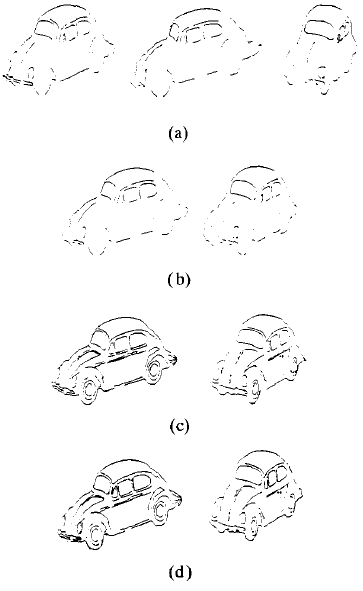
\includegraphics[height=0.6\textheight]{thesis/1991_JNL_TRKsub_Ullman_fig3.png}
								\caption{(a) Original images, (b) Synthetic images created from linear combinations of original images, (c) More original images at approximately same orientation as the synthetic images, (d) Synthetic images superimposed on original images~\cite{1991_JNL_Recog_Ullman}}.
								\label{fig:1991_JNL_TRKsub_Ullman_fig3}
								\end{figure}

In this work, we do not focus on the multi-camera approach.  We start our discussion with the VBR approach and transition to the online appearance approach for two reasons: (a) it historically predates the online appearance approach, and (b) it naturally leads to the online appearance approach.

In order to classify or recognize complex articulated objects, a large range of appearances are required.  One approach has been to use interpolation of appearance from a small number of views.  \cite{1991_JNL_Recog_Ullman} makes the assumption that all possible views of an object after 3D transformations such as rotation, translation and scaling can be expressed as the linear combination of other views of the same object.  Therefore, object matching is done by finding the distance between the linear subspace (or low dimensional manifold) defined by previous views and an observed object, rather than measuring the distance between the object and each of the stored views.  Figure~\ref{fig:1991_JNL_TRKsub_Ullman_fig3} shows an example of generating different car views using linear combinations of existing views.  



								\begin{figure}[t]
								\center
								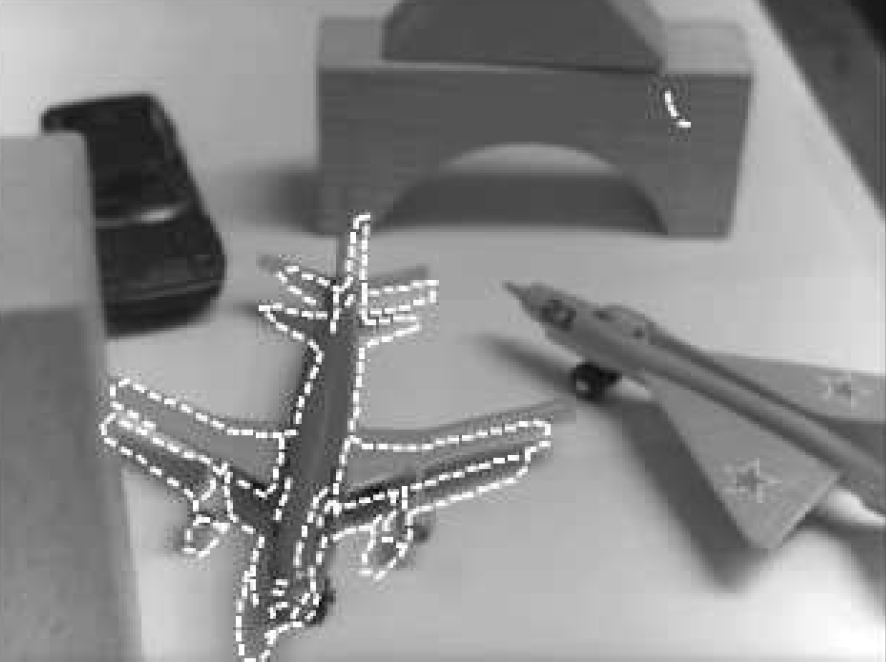
\includegraphics[width=0.6\textwidth]{thesis/1992_JNL_VBR_Breuel_fig1.png}
								\caption{Airplane recognized by view-based recognition system \cite{1992_JNL_VBR_Breuel}}
								\label{fig:1992_JNL_VBR_Breuel_fig1}
								\end{figure}

A generalization to this approach points out that exact representations do not always exist for continuous functions in terms of simpler functions~\cite{1990_JNL_Network_Poggio}.  However, good and general approximating representations may exist.  For instance, interpolation can be used for hypersurface reconstruction.  Since this problem is ill-posed, i.e. generally there's not enough data for a unique reconstruction, various assumptions such as smoothness are made.  These forms of regularization can be justifed using Bayesian MAP estimation.  A theoretical framework is then developed based on regularization techniques to create a three-layer network called a \emph{regularization network} which is useful for approximation, such as interpolation.

A step forward in the justification of view-based representations is presented in  \cite{1992_JNL_VBR_Breuel}, where it is shown that 300 views need to be stored for each view-based model to achieve an error rate smaller than that of optimal 3D matching algorithms.  An example of such a matching is shown in Figure~\ref{fig:1992_JNL_VBR_Breuel_fig1}.%In these experiments, 1000 images of bent paper clips were used, each paper clip being represented by 20 line segments.  The system developed was then used to recognize real world 3D objects from several Canny edge detection generated 2D views.

A fundamental question here is how to learn an appropriate set of view models.  As mentioned earlier, in traditional tracking approaches, such as normalized correlation or template matching, there is a limitation that the image motion must be simple, such as translation and the viewpoint must be fixed or changing slowly.  \cite{1993_CNF_Gestures_Darrell} tackle this challenge by using sets of view models, rather than simple templates.  In this approach, a data-driven method of using normalized correlation scores to automatically construct a set of view models is developed.  One initial model is specified by the user using a cursor.  The target object is tracked using normalized correlation.  The search function correlation scores are saved so that when they fall below a certain threshold, a new model can be added to the search set using the image at the offset with the best current score.  Over time, a family of view models that sample the aspect space are accumulated.  Two thresholds are maintained, one for deciding if track has been lost, and the other sets the level at which a new model should be added.  This method is then used to recognize human gestures.

								\begin{figure}[t]
								\center
								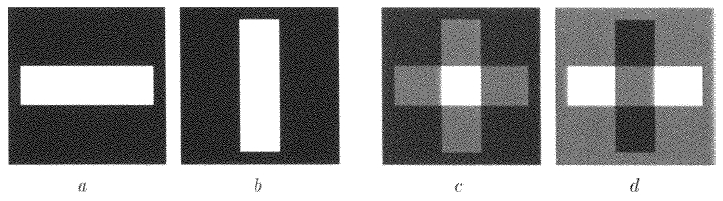
\includegraphics[width=1.0\textwidth]{thesis/TrackingPapers_SubspaceTracking_1998_Black_fig2_nocaption.png}
								\caption{(a, b) Training images (c, d) Eigenspace basis images \cite{1998_JNL_Eigentracking_Black}}
								\end{figure}


								\begin{figure}
								\center
								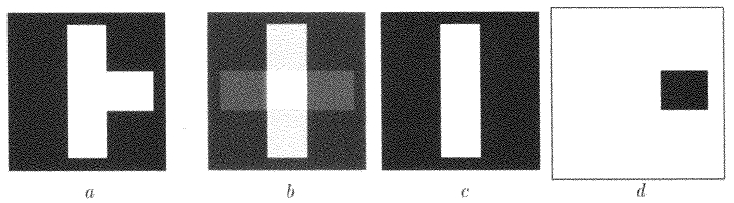
\includegraphics[width=1.0\textwidth]{thesis/TrackingPapers_SubspaceTracking_1998_Black_fig3_nocaption.png}
								\caption{(a) Test image (b) Least squares reconstruction (c) Robust reconstruction \cite{1998_JNL_Eigentracking_Black}}
								\end{figure}

A multi-view method that deals with illumination changes, to which SSD (sum of squared differences) or correlation based tracking is sensitive to, is presented in \cite{1996_TRK_region_Hager}.  A set of 5 basis images is created offline for a single face under a single view but different illumination conditions.  Images with maximum singular values in the SVD decomposition are retained for the basis.  These basis images are then used to approximate the object under any illumination condition.  This work also accounts for geometric changes in the face through affine warping.  

The transition of VBR to view-based tracking is first made in the seminal work of \emph{eigentracking} presented in \cite{1998_JNL_Eigentracking_Black}.  This is an adoption of initial work in the area of PCA based methods to efficiently represent several views \cite{1995_JNL_ActiveModels_Cootes, 1991_CNF_Eigenfaces_Turk}.  Before this work, eigenspace representations had focused on the problem of object recognition and had only peripherally addressed the problem of object tracking over time.  Additionally, it was assumed that the object of interest could be located in the image, segmented and transformed into canonical form for matching with the eigenspace.  However, this is not always possible and eigenspace reconstruction methods are not invariant to image transformations such as translation, scaling and rotation.  Two primary observations are made in this work that have formed the basis of current subspace tracking methods:

								\begin{figure}[t]
								\center
								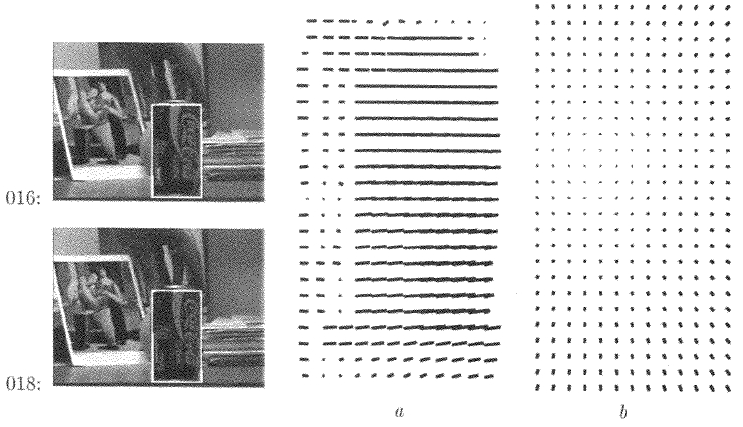
\includegraphics[width=1.0\textwidth]{thesis/TrackingPapers_SubspaceTracking_1998_Black_fig11_nocaption.png}
								\caption{Brightness versus subspace constancy.  "Motion" between frames 16 and 18 ( computed within the white boxed region) (a) dense optical flow for the soda can computed using the brightness constancy assumption (b) "Flow" computed using the subspace constancy assumption for the same frames \cite{1998_JNL_Eigentracking_Black}}
								\end{figure}


\begin{figure}[t]
\centering	
\subfigure[Training image.]{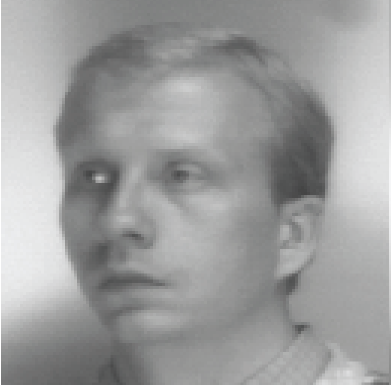
\includegraphics[width=0.3\textwidth]{thesis/TrackingPapers_SubspaceTracking_1997_Moghaddam_fig13_trginp.png}}
\subfigure[Training image reconstruction, parametric eigenspace]{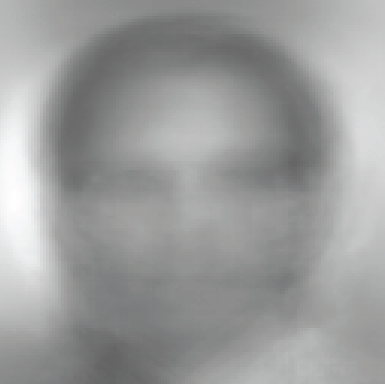
\includegraphics[width=0.3\textwidth]{thesis/TrackingPapers_SubspaceTracking_1997_Moghaddam_fig13_trgout_paramPCA.png}}	
\subfigure[Training image reconstruction, view-based eigenspace]{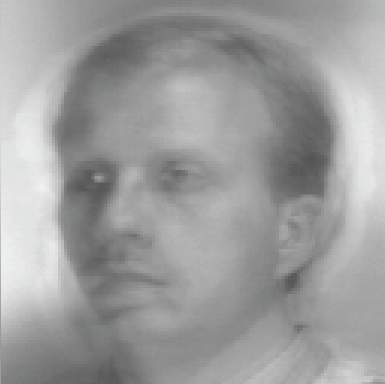
\includegraphics[width=0.3\textwidth]{thesis/TrackingPapers_SubspaceTracking_1997_Moghaddam_fig13_trgout_viewPCA.png}}	
\subfigure[Test image.]{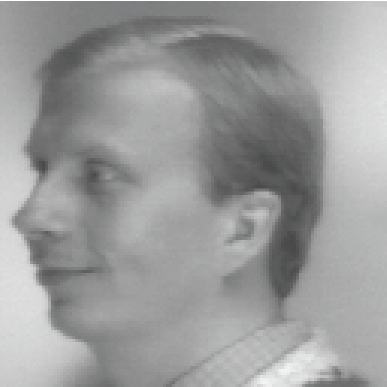
\includegraphics[width=0.3\textwidth]{thesis/TrackingPapers_SubspaceTracking_1997_Moghaddam_fig13_tstinp.png}}	
\subfigure[Test image reconstruction, parametric eigenspace]{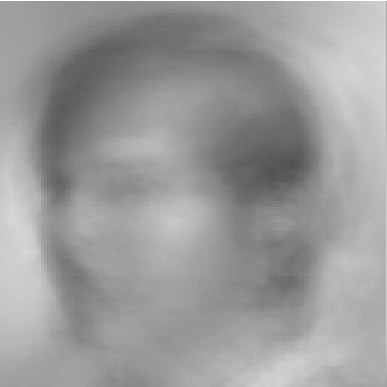
\includegraphics[width=0.3\textwidth]{thesis/TrackingPapers_SubspaceTracking_1997_Moghaddam_fig13_tstout_paramPCA.png}}	
\subfigure[Test image reconstruction, view-based eigenspace]{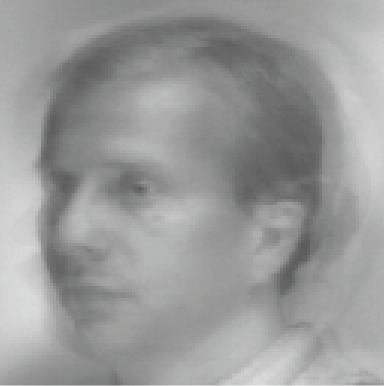
\includegraphics[width=0.3\textwidth]{thesis/TrackingPapers_SubspaceTracking_1997_Moghaddam_fig13_tstout_viewPCA.png}}	
\caption{Comparing parametric eigenspace with view-based eigenspace.}								
\label{fig:parametric_vs_viewBased_eigenspace}				
\end{figure}

\begin{enumerate}
\item \underline{Robust estimation.}  PCA reconstruction relies on a least squares fit between an image and the eigenspace.  This can lead to poor results in the presence of structured noise.  This work reformulates the eigenspace matching problem as one of robust estimation.
\item \underline{Affine transformation.} Instead of storing all views of the object to be tracked or learn interpolating surfaces in the eigenspace, an affine transformation is allowed between the input image and the subspace.
\end{enumerate}

A fundamental issue of whether to create one eigenspace for all classes or one eigenspace per class is addressed in~\cite{1997_JNL_EigenTRK_Moghaddam}.  The classes correspond to $M$ human head orientations with $N$ examples in every class.  In a \emph{parametric} eigenspace, one eigenspace is created for all $NM$ images.  On the other hand, in a \emph{view-based} eigenspace, one eigenspace is created for each of $M$ head orientations, each with $N$ users per eigenspace.  Since multiple views of a face form a connected non-convex region \cite{1994_JNL_FaceTop_Bichsel}, the analogy of using a parametric versus a view-based eigenspace approach is that of modeling a complex distribution by a single cluster model or the union of several component clusters respectively.  It is expected that the latter approach will give better image reconstruction results and that is seen in Figure~\ref{fig:parametric_vs_viewBased_eigenspace}.  

The state of the art in subspace tracking is presented in \cite{2008_JNL_subspaceTRK_Ross}.  In this work, the authors initially create an offline eigenbasis.  Subsequent images are added using an incremental PCA update with a forgetting factor to update the eigenbasis every 5 frames.  They use a particle filter for motion parameter estimation.  Pose, expression, lighting, temporary occlusion and structured appearance changes are all addressed and tracked successfully.

In \cite{2003_JNL_TRKsubspace_Jepson}, phase is chosen as the basis of the appearance model since it provides some amplitude and illumination independence.  They compute the optimal image warp from the stable properties of image appearance.  They develop a $\mathcal{WSL}$ tracker, where $\mathcal{S}$ rerers to the stable component, $\mathcal{L}$ refers to the "lost" component, and $\mathcal{W}$ refers to the wandering component.  The $\mathcal{S}$ component captures the behavior of the stable and slowly varying image observations when and where they occur.  The $\mathcal{L}$ component accounts for data outliers which arise as a result of tracking failures due to tracking, occlusion, or noise.  The $\mathcal{W}$ component allows for adaptation to short term image appearance changes.  A mixture model is used to model these 3 components.  The image feature used to generate the mixture model is the phase.  The model is learned online using the EM algorithm.  This method can handle variations in pose, illumination and expression.  However, since pixels are treated independently, within the target region, a notion of an object being tracked does not exist.  This can result in modeling the background as well. 

								\begin{figure}[t]
								\centering	
								\subfigure[In the image on the right, dimension is fixed to 50]{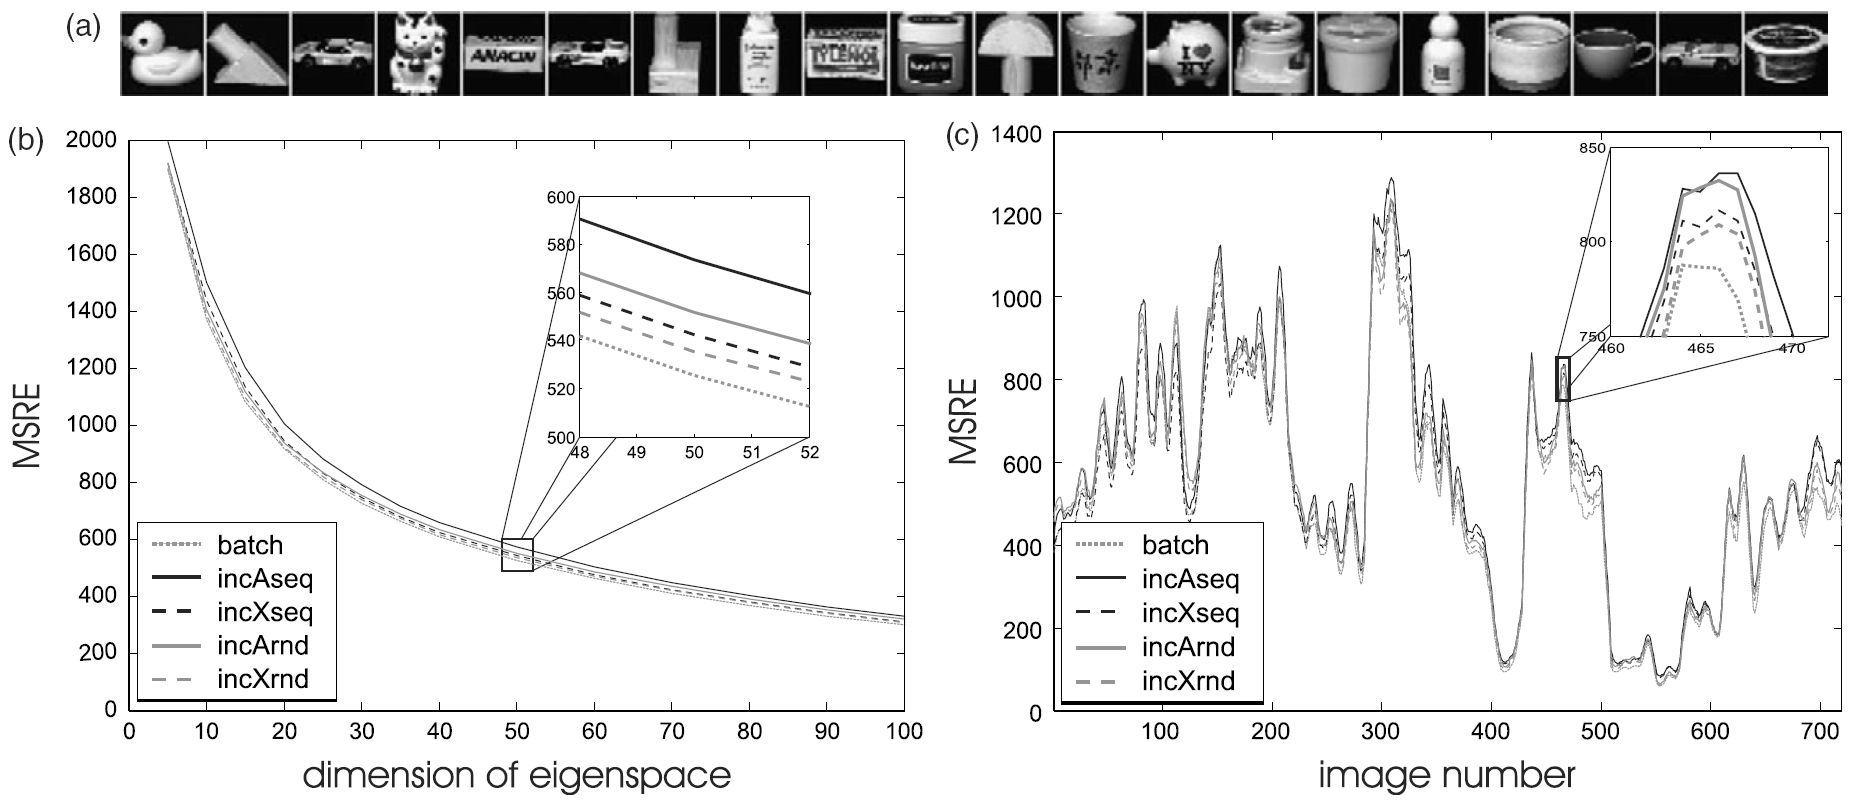
\includegraphics[width=1.0\textwidth]{thesis/2008_JNL_TRKsub_Skocaj_fig4.png}}
								\subfigure[Comparison of weighted vs non-weighted batch and incremental PCA algorithms]{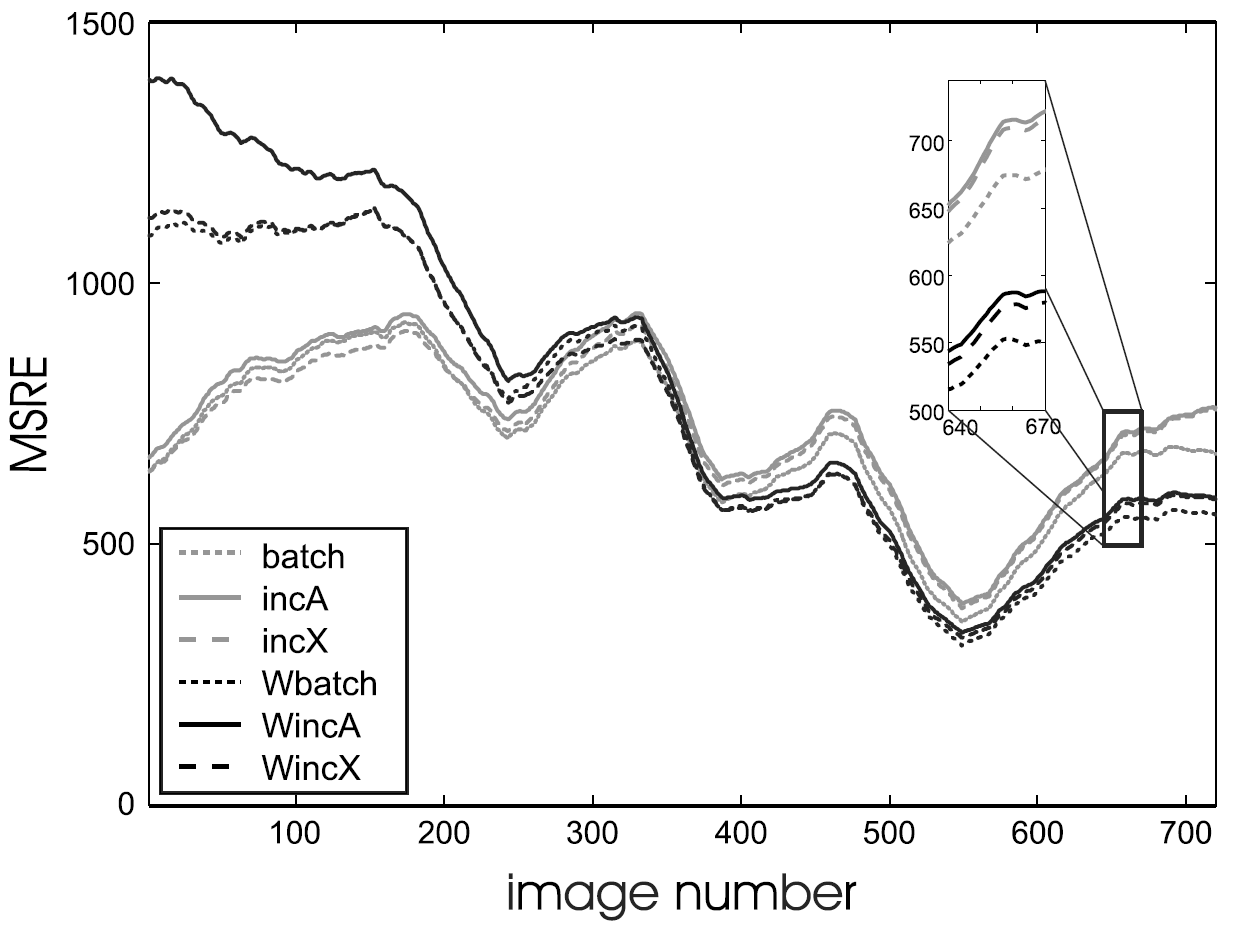
\includegraphics[width=0.5\textwidth]{thesis/2008_JNL_TRKsub_Skocaj_fig5.png}}
								\caption{Comparison of batch PCA with various incremental PCA update algorithms \cite{2008_JNL_TRKsubs_Skocaj}}
								\label{fig:2008_JNL_TRKsub_Skocaj}				
								\end{figure}

\cite{2008_JNL_TRKsubs_Skocaj} try to find the error associated with using an incremental PCA update algorithm versus using the optimal batch PCA algorithm.  They build eigenspaces of various dimensions from 720 images of 20 objects taken from the Columbia University Image Library (COIL-100)  \cite{Web_COIL}.  Figure~\ref{fig:2008_JNL_TRKsub_Skocaj} shows the mean squared reconstruction errors (MSRE) for the batch and various incremental methods.  In all experiments, squared reconstruction error degradation is less than 10\%.  Moreover, the sequential order in which the images are presented influences results.  It is pointed out that to obtain good results, the initial images should be heterogenous encompassing different objects and views.  This results in an evolving eigenspace that is rich and comprehensive enough in the beginning and is not specialized for representing a specific object only.  In this work, it is also shown that the reconstruction errors of the various incremental weighted PCA methods (\emph{WincA, WincX}) do not differ significantly from the results of the batch weighted method (\emph{Wbatch}).  This method is used by \cite{2010_CNF_TRKsubs_Qian} for object tracking in a manner quite similar to the approach used in \cite{2008_JNL_subspaceTRK_Ross}.  They sample a collection of image patches and likelihood of each image patch is generated by reconstruction.  Comparison is made between PCA subspace tracking with and without weighting prior observations.  They show that temporal weighting the data results in less background clutter penetrating the target of interest and therefore leads to better occlusion handling in tracking.  Another incremental PCA update algorithm is developed by \cite{2004_JNL_TRKsubs_Li}.  They also propose an incremental algorithm robust PCA in addition to standard PCA.

Having discussed traditional and subspace based tracking methods, we now turn to the usage of RVQ in tracking.


%								\begin{figure}[t]
%								\center
%								\includegraphics[width=0.5\textwidth]{thesis/PRML_hierarchy_Bayes_MRF_regularization.pdf}
%								\caption{Splines are equivalent to standard (smoothness based) regularization.  Standard regularization is a special case of MRF models.  MRF models are a subset of Bayesian estimators \cite{1990_JNL_Network_Poggio}}
%								\label{fig:PRML_hierarchy_Bayes_MRF_regularization}
%								\end{figure}

%\end{Body}
%%##############################################################################################################
%\begin{EndMatter}
%\references 				%generates the bibliography page
%\end{EndMatter}
%\end{document}
%%##############################################################################################################
